\chapter{Indledning} 
Ved ultralydsscanning af gravide er arbejdsgener hos sonograferne et kendt problem. For at udføre scanningerne holder sonograferne proben i akavede stillinger, der udsætter deres skulder, arm og håndled for store belastninger \cite{1}\cite{24}\cite{31}\cite{32}\cite{36}. Disse belastninger forøges, når et pres på mellem 3 og 11 kilogram kræves for at få et klart ultralydsbillede, se Bilag 12, 28.04.2016. Disse stillinger øger risikoen for at få arbejdsgener, der med tiden kan føre til arbejdsskader. Grundet sonografernes belastende arbejdsstillinger er der fra Dansk Føtalmedicinsk Selskab opstillet guidelines angående det maksimale antal timer, en sonograf anbefales at foretage scanninger i løbet af en uge. Disse guidelines er på 28 timer om ugen, se Bilag 10. Dette gør, at der skal flere sonografer til for at kunne scanne det stigende antal gravide i Danmark \cite{Foedsler}. \\
Samtidig er Danmark under en udvikling, der gør at antallet af overvægtige kvinder stiger \cite{Overvaegt}. Dette gør, at sonograferne skal presse med en større kraft for at få billeder af tilsvarende kvalitet, se Bilag 12, 28.04.2016,\cite{24}\cite{31}\cite{8}. 

Gennem en årrække er der lavet en række forskningsstudier og forsøg med robotarme til ultralydsscanning af hjertet for at aflaste scanningspersonalet \cite{5}. Dette er med til at underbygge, at problemstillingen er kendt, men den optimale metode er endnu ikke fundet. Yderligere findes der flere forskningsstudier, der omhandler udviklingen af robotter til lignende opgaver \cite{8}\cite{5}\cite{18}. 

Denne udvikling har ført til, at firmaet Robotic Ultrasound ApS er i færd med at udvikle en Ultralyds Robotarm, der forventes at kunne afhjælpe problemet. Denne robotarm styres via et joystick, således at sonograferne kan undgå de akavede arbejdsstillinger, se figur \ref{opstilling}.  

\begin{figure}[H]\centering
	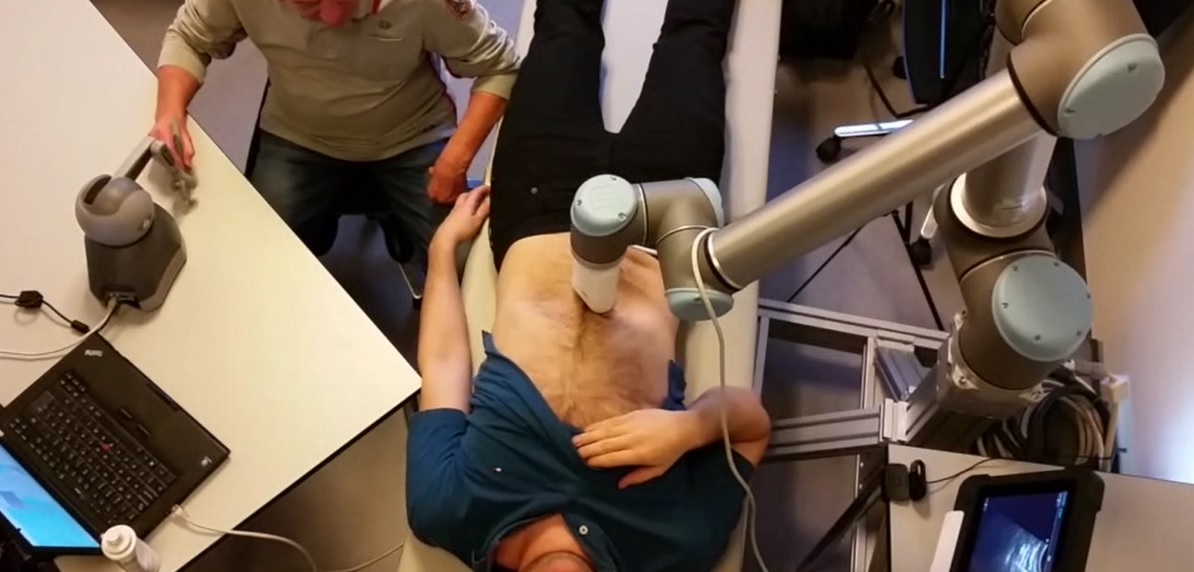
\includegraphics[width = 0.85\textwidth]{Figurer/ergonomiskLosning.jpg}
	\caption{Eksempel på opstilling af Ultralyds Robotarm. På billedet ses joystick (tv.) og robotarm (th.).  }
	\label{opstilling}
\end{figure}

%Problemstillingen i denne form er et område der ikke tidligere er afdækket. Men tidligere forskning i forhold til ultralydsscanning med robot gør at der findes tilstrækkelig videnskabelig dokumentation til at bygge mini-MTV’en op omkring. 

\section{Formål}
Formålet med denne mini-MTV er derfor at vurdere, om Ultralyds Robotarmen kan implementeres som en teknologisk aflastning for sonografer i deres arbejde med scanning af gravide. Det ønskes at klarlægge fordele og ulemper ved de eksisterende arbejdsforhold og ved implementering af Ultralyds Robotarmen, samt hvilke forskelle robotarmen vil medføre for sonografer og gravide. \\
Dette vil blive undersøgt ved at besvare følgende opstillede MTV-spørgsmål i rapporten:
\begin{itemize}
\item Hvilke funktioner har teknologien og hvordan anvendes teknologien?
\item Hvilke arbejdsgener oplever sonografer under ultralydsscanning ved eksisterende procedurer og hvorledes påvirkes dette ved indførsel af teknologien?
\item Hvorledes vil afdelingernes arbejdsgange blive påvirket ved indførsel af teknologien?
\item Hvilke etiske og patientmæssige udfordringer vil der være ved at indføre teknologien?
\item Hvad vil de økonomiske konsekvenser være ved at indføre teknologien i forhold til eksisterende procedurer?
\end{itemize}

Yderligere forventes det, at rapportens resultater vil blive efterspurgt forud for en beslutningstagning, når robotarmen er færdigudviklet og produceret. Dermed er formålet med mini-MTV’en også at bidrage til beslutningsgrundlaget for den enkelte sygehusafdeling, samt hvilke aspekter, der skal tages højde for og medtages i en vurdering.

\section{Projektafgrænsning}
Projektet afgrænses til en vurdering af, hvorvidt der er tilstrækkeligt grundlag til at gøre brug af en Ultralyds Robotarm ved scanning af gravide i forhold til det udstyr, der benyttes på afdelingerne i dag. Det primære fokus i projektet er problemstillingen, at et stort antal sonografer oplever arbejdsgener under scanningsarbejdet \cite{1}\cite{24}\cite{31}\cite{36}\cite{30}. \\
Rapportens fokus på sonografer er fundet ved udarbejdelse af interessentanalyse, se Bilag 14. Projektet blev afgrænset til dette fokus, da sonografer er den personalegruppe, der foretager størstedelen af scanningerne af gravide, se Bilag 4 og Bilag 5.

Ultralyds Robotarmen åbner for muligheden om at bruge denne som en telemedicinsk løsning, hvor sonografen er placeret andetsteds. Dette aspekt er fravalgt grundet begrænset omfang af denne mini-MTV. 

Opgaven er afgrænset til en 25 siders mini-MTV, hvor det skriftlige omfang på en typisk dansk MTV ligger på over 100 sider \cite{Leavitt}. I en mini-MTV vurderes problemstillingen på de fire parametre: Teknologi, Organisation, Patient og Økonomi. 

Den korte tidshorisont til udarbejdelsen af denne mini-MTV har været en afgørende faktor for, at det er valgt at begrænse projektet til at bygge på interview med to relevante danske sygehusafdelinger, samt en litteratursøgning på problemstillingen. Interviews er afholdt med "Kvindeafdelingen, Svangre- og Ultralydsambulatorium" på Hospitalsenheden Horsens (HEH) og afdelingen "Kvindesygdomme og Fødsler" på Regionshospitalet Viborg (RMV).

\section{Projektorganisation}
Projektet er blevet udarbejdet som semesterprojekt af seks sundhedsteknologistuderende på 4. semester ved Aarhus Universitet Ingeniørhøjskolen. \\
Hovedforfattere til de enkelte kapitlerne er:
\begin{itemize}
\item Teknologi: Ditte Callesen, Ida Skovbjerg og  Mette Knudsen
\item Organisation: Anne Hoelgaard, Ida Skovbjerg og Nina Brkovic
\item Patient: Ditte Callesen, Freja Munk og Nina Brkovic
\item Økonomi: Anne Hoelgaard, Freja Munk og Mette Knudsen
\end{itemize}

\label{version_Systemark}
%\end{longtabu}